\section{\esp Introdução}
Com a mudança de mentalidade da Web para o novo paradgma de aplicações web conhecido como Web 2.0 proposta por \cite{web20Proposta}, seus 
usuários deixaram de ter um papel passivo como consumidores de conteúdo para assumir um papel ativo de produtores de conteúdo. Esta mudança 
trouxe consigo ferramentas interativas, que tem como foco principal a geração de conteúdo por parte dos próprios usuários, tais como fóruns 
de discussões e recentemente, as redes sociais como o Twitter, Facebook e o Instagram.

Esta participação ativa dos usuários impactou significativamente a quantidade de informação disponíveis na Web. Segundo \cite{artigo01}, 
o tráfego de dados nesta rede dobra a cada ano, o que gera uma quantidade massiva de informação, tornando a Web muito influente em diversos 
setores de grande importância na sociedade, passando a fazer parte do cotidiano das pessoas que estão cada vez mais conectadas a mecanismos que
as  conectam aos conteúdos de seu interesse. Podemos perceber esta influência principalmente através das redes sociais, que segundo 
\cite{redesSociais01} estão mudando profundamente as formas de organização, identidade, conversação e mobilização social.

Como descreve \cite{deitelAjax}, com todo este conteúdo disponível, os mecanismos de busca de informação 
acabam recebendo destaque nesta ``nova Web'' e sobressaem aqueles que auxiliam os usuários  a localizar e filtrar 
as informações desejadas. Desta forma, há um grande desafio em relação à formulação de ferramentas que guie o usuário até os conteúdos de seu 
interesse, economizando assim sua atenção. Estas ferramentas com o passar do tempo se fazem mais presentes no dia-a-dia das pessoas, 
que por sua vez demandam por mecanismos cada vez mais robustos e personalizados de acordo com suas necessidades, como consequência existe 
uma demanda constante de novas aplicações mais específicas para atender determinada comunidade.

No estudo estudo realizado por \cite{perfilCicloturista}, após realizar uma pesquisa com 302 cicloturistas, concluiu-se que a internet é sem dúvidas 
o meio de informação mais utilizado por esta comunidade, totalizando 46\% das respostas em relação à qual o meio de informação utilizado por eles.
No entando, neste meio há uma demanda ainda não explorada por uma aplicação focada nesta prática, pois de acordo com \cite{cicloturismo02}, 
as grandes viagens realizadas sobre a bicicleta requerem um melhor preparo e conhecimento, por parte do ciclista, e ressalta a importância de se 
conhecer a extensão da viagem e tempo total disponível, além da região, relevo e clima escolhidos como trajeto. Devido a complexidade do planejamento
requerido, percebe-se neste meio a necessidade de uma ferramenta que centralize informações importantes para tal. Praticantes desta atividade por não 
possuírem uma ferramenta específica, recorrem a outras com propósito similares para auxiliá-los no planejamento de seus trajetos, que não oferecem 
informações importantes para este planejamento. O cicloturismo conforme descrito por \cite{cicloturismo01} é uma modalidade do ecoturismo que está 
ganhando cada vez mais adeptos no Brasil, por ser uma atividade de baixo impacto ambiental, já que é realizado com bicicletas.

Este trabalho tem como objetivo desenvolver uma ferramenta no formato rede social Web voltada a atender esta demanda de informações observada 
no meio do cicloturismo. Segundo \cite{perfilCicloturista} o  "fenômeno" cicloturismo é considerado de fraco a bom em termos de comunicação 
e estrutura para receber os cicloturistas. Com o Ciclotour, visamos prover um meio de comunicação onde usuários desta ferramenta terão acesso de 
forma centralizada a informações sobre rotas que pretendem trilhar, fornecidas por outros usuários de forma colaborativa, com o propósito 
de criar um grande repositório de informações relevantes para cicloturistas auxiliando no planejamento da atividade turística, comunicação entre 
praticantes e promoção da prática.

\section{\esp Referencial Teórico}
No princípio das aplicações Web, devido ao seu comportamento síncrono, as mesmas ficaram para trás em relação a aplicações \textit{desktop}, pois a 
interação com essas aplicações resultava em um longo período de espera conforme descreve \cite{deitelAjax}. Este atraso era causado devido à grande 
quantidade de atualizações de páginas inteiras necessárias no ciclo síncrono, demonstrado na Figura \ref{fig:arquitetura_web_tradicional}. 

\begin{figure}[!ht]
	\centering	
	\caption[\hspace{0.1cm}Aplicação Web clássica.]{Aplicação Web clássica}
	  \vspace{-0.4cm}
	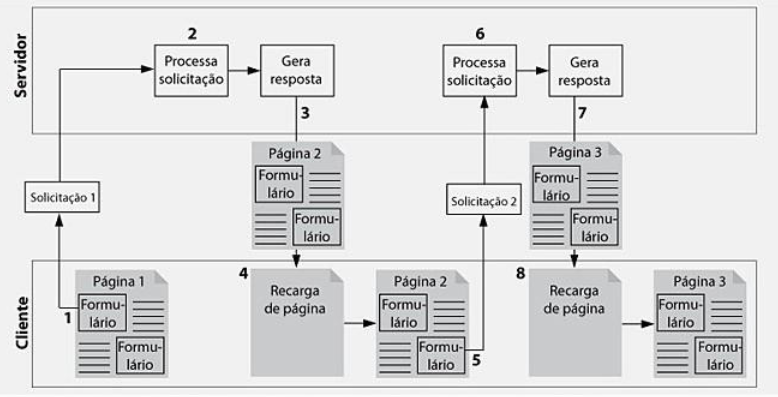
\includegraphics[width=.8\textwidth]{figuras/arquitetura_web_tradicional.png}
	 \vspace{-0.3cm}
	\\\textbf{\footnotesize Fonte: \cite{deitelAjax}}
	\label{fig:arquitetura_web_tradicional}
\end{figure}

Cada recarga na página gerava uma nova requisição ao servidor, que neste modelo é responsável por processar a requisição, gerar e enviar a resposta 
contendo a página exata que será exibida no \textit{browser} do cliente. Esse \textit{delay} presente nas interações com a aplicação fizeram com que 
os usuários ``exigissem'' uma forma melhor de interagir com estas aplicações. 

Para solucionar este problema de desempenho presente nas aplicações tradicionais, surgiu o modelo Ajax. Como descrito por \cite{garrettAjax}, uma 
aplicação Ajax elimina a natureza de interação Web conhecida como \textit{start-stop-start-stop} introduzindo uma camada intermediária 
— \textit{Ajax Engine} — entre cliente e servidor. Essa camada permitiu a essas aplicações realizarem requisições ao servidor de forma assíncrona 
e atualizar parcialmente a página ao receber a resposta, não impedindo a interação do usuário durante o ciclo de requisição/resposta. Na 
Figura \ref{fig:ajax_comparison} podemos ver um comparativo entre aplicações Web síncronas e assíncronas.

\begin{figure}[!ht]
	\centering	
	\caption[\hspace{0.1cm}Comparação aplicação Web clássica e aplicação Web com Ajax.]{Comparação aplicação Web clássica e aplicação Web com Ajax}
	  \vspace{-0.4cm}
	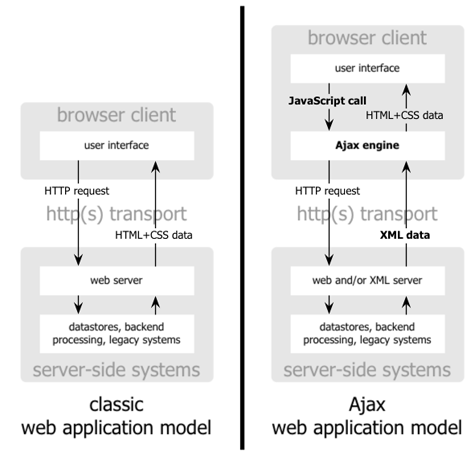
\includegraphics[width=.6\textwidth]{figuras/ajax_comparison.png}
	 \vspace{-0.3cm}
	\\\textbf{\footnotesize Fonte: \cite{garrettAjax}}
	\label{fig:ajax_comparison}
\end{figure}


Com aplicações construídas utilizando Ajax, a Web voltou à ser atrativa para usuário e tem crescido o número de aplicações Web desde então. Segundo
\cite{tabulaRest} as aplicações Web assumem atualmente uma importância sem precedentes em todas as áreas da sociedade. 

Em \cite{fieldingRest} foi apresentado o \textit{Representational State Transfer} (REST) como um estilo arquitetural para sistemas de hipermídia 
distribuídos baseado no \textit{HyperText Transfer Protocol} (HTTP). Segundo \cite{modelingRestful}, o entendimento do REST pode ajudar na obtenção 
de uma melhor performace e escalabilidade, bem como diminuir o acoplamento, como resultado aumentando a interoperabilidade, promovendo o reuso. 
Aplicações que seguem as restrições REST são denominadas como RESTful, estas aplicações consistem em um \textit{Web Service} simples que utiliza 
verbos HTTP para mapear ações as \textit{Create, Read, Update, Delete} (CRUD). Podemos ver na Tabela \ref{tab:tabela1} o mapeamento de verbos HTTP 
com as ações CRUD.

\begin{table}[htb]
	\centering
	\caption{\hspace{0.1cm} Relacionamento de verbos HTTP com ações CRUD}
	\vspace{-0.3cm} % espaço entre titulo e tabela
	\label{tab:tabela1}
	% Conteúdo da tabela
	\begin{tabular}{l|c}
  \hline
    \textbf{HTTP} & \textbf{Ação} \\
    \hline
      GET & Read \\
      POST & Create \\
      PUT & Update \\
      DELETE & Delete \\
     \hline
 \end{tabular}
 	\vspace{.1cm}  %espaço entre tabela e fonte
	\small
	% Fonte
	{\footnotesize\\ \textbf{Fonte: Elaborado pelo autor}}
\end{table}

Devido a este aprimoramento constante no que diz respeito ao desenvolvimento de aplicações Web, a arquitetura de uma aplicação Web está deixando 
de ser composta por grandes quantidades de códigos \textit{server-side}, onde todo o processamento é feito no servidor, os códigos são fechados e 
o consumo de banda é maior aos proprietários do sistema, e passando a ter maior utilização de códigos \textit{client-side}, onde o processamento dos 
\textit{scripts} da página ocorre na máquina do cliente e somente quando há necessidade de interação com o banco de dados são feitas requisições ao 
servidor \cite{spa01}. Neste contexto surgiram as \textit{Single Page Applications} (SPA) definida por \cite{spa02} aplicações composta por somente 
uma página HTML, como base para todas as outras páginas Web da aplicação nas quais as interações feitas pelo usuário são implementadas usando 
JavaScript, HTML e CSS. A Figura \ref{fig:spa} demonstra o funcionamento de uma SPA.

\begin{figure}[!ht]
	\centering	
	\caption[\hspace{0.1cm} Ciclo de vida de uma Single Page Application.]{Ciclo de vida de uma Single Page Application}
	  \vspace{-0.4cm}
	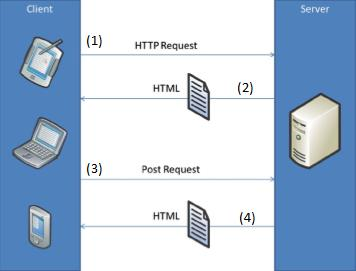
\includegraphics[width=.6\textwidth]{figuras/spa.png}
	 \vspace{-0.3cm}
	\\\textbf{\footnotesize Fonte: \cite{spa02}}
	\label{fig:spa}
\end{figure}

Em aplicações SPA, a primeira requisição realizada pelo cliente recebe como resposta uma página HTML, nesta página inicial há um extenso conteúdo de
\textit{scripts} responsáveis pela navegação do usuário, sem que haja recarga da página, quando há necessidade de conteúdos presentes no servidor, 
esta comunicação é feita através de requisições Ajax, e os scripts presentes na página são responsáveis por renderizar estes conteúdos recebidos na
página, através do \textit{Document Object Model} (DOM). Toda transição de páginas neste tipo de aplicação é realizada \textit{client-side}. 
Uma das vantagens da adoção deste modelo em relação ao modelo anterior é em relação ao \textit{overhead} de requisições, o que torna a aplicação 
mais leve e permite melhor usabilidade para o usuário final, devido ao AJAX não bloquear a manipulação da página durante sua execução \cite{spa01}, 
além de facilitar a portabilidade da aplicação pois este modelo requer uma API \textit{server-side} robusta e bem estruturada para funcionar.

\section{Trabalhos Relacionados}
\subsection{Runtastic}
A rede Runtastic \cite{runtastic}, reúne várias modalidades de esportes como ciclismo, corrida ou triatletismo. Oferece à seus usuários a
possibilidade de registrar suas atividades e performace obtida, afim de montar estatísticas que podem ser compartilhadas com seus amigos e usadas 
para medir seu progresso. Esta rede social está associada à várias práticas físicas, com seu foco voltado ao treinamento. É munida de estatísticas 
para auxiliar em análises de desempenho de atletas em geral e não somente ciclistas. Suas rotas tem como finalidade demarcar o trajeto e progressos 
físicos em rotinas de treinos. As funções desta rede não abrangem atividades turísticas. Esta rede possui o recurso de enviar fotos de momentos 
durante sessões de atividades físicas realizadas pelo usuário. A rede  possui duas opções de idiomas inglês e alemão. Permite utilizar aplicativo 
\textit{mobile} para acompanhamento e GPS para gerar as estatísticas com base na atividade realizada. Como recursos de rede social, o Runtastic 
permite relacionamento de amizade entre usuários, \textit{post's} no mural de outros usuários, acompanhamento em tempo real através de um mapa a 
atividade realizada por outros usuários, enviar \textit{cheer's} para o usuário que está realizando a atividade, além de comentários sobre a 
atividade realizada e dar \textit{like} na mesma. 

\subsection{Strava}
A rede Strava \cite{strava} possui diversas funções voltadas à prática de atividades físicas diárias, focadas em caminhadas/corridas e ciclismo. Esta
rede possibilita seus usuários ao redor do mundo registrarem seus esforços físicos diariamente, pois possui um registro de atividades físicas visando 
comparar o seu progresso. Oferece à seus usuários desafios para estimula-los a aumentar sua performance, possui o recurso de traçar rotas com o 
objetivo de planejar a atividade esportiva e treinamento. Nesta rede é possível cadastrar metas personalizadas relacionadas à desempenho, 
possibilitando seus usuários um acompanhamento de seu progresso em suas atividades, além possuir quadros informativos sobre distâncias percorridas 
em relação à espaços de tempo. Como recursos de rede social, o Strava permite ao usuário seguir outros usuários, ingressar em grupos de usuários 
denominados clubes que podem ser públicos ou privados, possui um feed de atividades onde são exibidas atividades realizadas por todos os usuários da 
rede, neste feed são exibidas fotos compartilhadas durante a realização destas atividades e a rota percorrida com informações de distância total e 
horário inicial e final da atividade. Esta rede possui um aplicativo mobile que registra através do uso do GPS a atividade do usuário e permite ao 
mesmo compartilhar fotos tiradas durante o percurso. O Strava não oferece nenhum recurso voltado à atividades turísticas.

No Quadro 1 podemos ver um quadro comparativo entre as funções do Ciclotour e das redes analisadas.

   \begin{center}
          \centering
       	\textbf{Quadro 1 - Comparação entre funcionalidades das Redes e o Ciclotour}\\
        \label{quadro1}
	\begin{tabular}{|c|c|c|} \hline
	\multicolumn{3}{|c|}{\textbf{Comparação entre funcionalidades das Redes e o Ciclotour }} 	  \\
		\hline \textbf{ Funções do Ciclotour } & Strava & Runtastic \\  
		\hline \textbf{ Criar rotas personalizadas } & SIM & SIM \\ 
		\hline \textbf{ Criar pontos informativos em rotas } & NÃO & NÃO  \\
		\hline \textbf{ Indicar tipo do terreno da rota } & SIM & SIM \\ 
		\hline \textbf{	Adicionar Fotos à Rota } & NAO & NAO \\ 
		\hline \textbf{ Comentários em rotas }	& NÃO & SIM \\ 
		\hline \textbf{	Comentários em pontos } & NAO & NAO \\ 
		\hline \textbf{	Marcar rotas como realizadas ou pendentes } & NAO & NAO \\ 
		\hline \textbf{	Permitir relação de amizade entre usuários } & NÃO & SIM \\ 
		\hline \textbf{	Buscar rotas com base em origem e destino } & NÃO & NÃO \\ 
		\hline
	\end{tabular}
	\vspace{0.1cm} 
	{\footnotesize\\ \textbf{Fonte: Elaborado pelo autor}}
   \end{center}

\section{Metodologia}
O ciclo de desenvolvimento da aplicação Ciclotour foi dividido nas seguintes fases: Coleta inicial de requisitos, teste de aceitação via 
\textit{mockup} por parte do fornecedor de requisitos, implementação das \textit{features} aceitas e teste final de aceitação. Para isso 
o desenvolvimento do Ciclotour contou com uma abordagem \textit{top-down}, nesta abordagem o \textit{front-end} é construído antes do 
\textit{back-end}. Foi adotada esta abordagem de desenvolvimento pois desta forma é possível aprovar o funcionamento do sistema à partir de um 
\textit{mockup} de como seria a usabilidade da tela, sem necessidade de implementar toda a aplicação. Assim, o ``custo'' de mudanças é reduzido, 
pois além do que foi contruído ter passado por uma pré-aprovação do fornecedor de requisitos, o maior custo de mudanças se dá em alterações de 
modelos de banco de dados, que só será implementado após aprovação, evitando que sejam necessárias este tipo de mudança. Desta forma é possível 
evitar retrabalho e ainda com este propósito, o sistema foi desenvolvido utilizando a técnica conhecida como \textit{Test Driven Development} (TDD), 
nesta técnica o desenvolvimento é guiado por testes, visando garantir que o que foi desenvolvido está correto. O ciclo de desenvolvimento do 
Ciclotour priorizou minimizar o retrabalho ao máximo devido ao curto período de tempo disponível.

\section{\esp Ferramentas}
Para o desenvolvimento do Ciclotour, foi utilizado o estilo arquitetural RESTful, sendo este sistema contruído como uma SPA. Desta forma, há
uma separação completa das responsabilidades entre cliente e servidor, onde a responsabilidade de composição das páginas é delegada ao browser
executado \textit{client-side} e o servidor passa a atuar apenas como um repositório dos dados pertinentes à aplicação. A Figura 
\ref{fig:estruturaCiclotour} demonstra a estrutura simplificada entre cliente e servidor da aplicação Ciclotour, e as tecnologias utilizadas para
a construção do sistema.

\begin{figure}[!ht]
	\centering	
	\caption[\hspace{0.1cm} Estrutura simplificada entre cliente e servidor da aplicação Ciclotour.]
	{Estrutura simplificada entre cliente e servidor da aplicação Ciclotour}
	  \vspace{-0.4cm}
	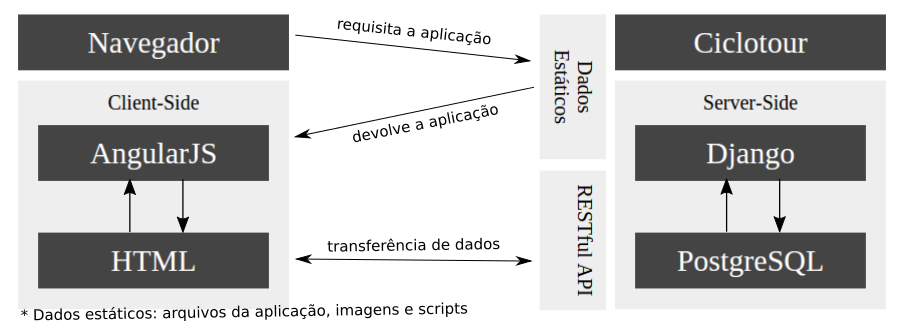
\includegraphics[width=1\textwidth]{figuras/estruturaCiclotour.png}
	 \vspace{-0.3cm}
	\\\textbf{\footnotesize Fonte: Elaborado pelo autor}
	\label{fig:estruturaCiclotour}
\end{figure}

\subsection{Servidor}
Para desenvolver o \textit{server-side} da aplicação Ciclotour foram utilizados o \textit{framework} Python de desenvolvimento Web Django com a 
extensão Django REST Framework para construção de \textit{Web Services}. O Django utiliza um estilo arquitetural baseado no 
\textit{Model-View-Controller} (MVC), o \textit{Model-View-Template} (MVT). Na aplicação Ciclotour o Django é responsável por processar a 
solicitação inicial onde a página contendo todos os \textit{scripts} necessários para a aplicação é devolvida como resposta para o solicitante,
manter uma interface de administração do sistema e manter os modelos do sistema através de seu \textit{Object-relational mapping} (ORM). 
As requisições posteriores enviadas ao servidor serão requisições de dados que serão processadas e respondidas pelo Django REST \textit{framework} 
em formato \textit{JavaScript Object Notation} (JSON).

\subsection{Cliente}
Para desenvolver o \textit{client-side} da aplicação Ciclotour foram utilizados o \textit{framework} JavaScript AngularJS e o \textit{framework} 
CSS Bootsrap. O AngularJS tem como propósito permitir a construção de elementos \textit{client-side} de forma declarativa, através de suas diretivas.
Este \textit{framework} também adota o estilo arquitetural MVC, além de prover uma abstração para as chamadas Ajax e atualização em tempo real do 
\textit{Document Object Model} (DOM) através do \textit{Two-way Data Binding}, o que promove uma melhor organização do projeto que por se tratar de
uma SPA, possui alto grau de complexidade em seus scripts. Devido à esta facilidade oferecida pelo \textit{framework}, o AngularJS foi utilizado 
desenvolver de todos os scripts \textit{client-side} da aplicação Ciclotour. O Bootstrap foi utilizado com o intuito de oferecer uma interface rica 
e com \textit{design} responsivo para promover melhor usabilidade e experiência por parte do usuário final do sistema.